\chapter{Modeling}\label{ch02}

Selective filters made of biopolymers are used in living and
synthetic systems to control the localization and movement of
molecules, nanoparticles, viruses and other organisms \cite{witten17}.
These filters regulate access to genetic material (the nuclear pore
complex, or NPC), cells (the pericellular matrix), tissues (the
extracellular matrix), and organs (mucus). In addition to their
protective role, polymeric biomaterials are physical barriers that can
inhibit drug delivery. Microbial biofilms can sequester antibiotics in
their pericellular matrix, hindering treatment of infections
\cite{hoiby10}. The extracellular matrix and mucosal layers limit drug
delivery in cancer and other diseases \cite{witten17}. How particle
binding affects motion and filtering is unclear. Binding to the
pericellular matrix facilitates uptake of nanoparticles by single
cells \cite{zhou12}, and transport factors that bind to proteins in
the NPC move rapidly through it \cite{strambio-de-castillia10}.  In
contrast, binding inhibits the uptake of nanoparticles that bind to
airway mucus \cite{schneider17, huang17, mastorakos15}. Many viruses
minimize binding interactions, allowing human papillomavirus and human
immunodifficiency virus to move nearly unrestricted in cervical mucus
under certain conditions \cite{olmsted01,lai09}, although antibody binding 
can slow these interactions \cite{chen14}.  Improved design of
drug delivery vehicles and synthetic selective filters requires
understanding what distinguishes these behaviors.  While particle
size, charge, and binding interactions are known to affect filtering
\cite{witten17}, the physical principles that underlie mobility and
transport in polymeric biomaterials are not fully understood.

Among these filters, the NPC is tuned for selective passage enabled by
binding.  The NPC selectively filters molecular traffic between the
nucleus and cytoplasm of eukaryotic cells, making it important for
diverse processes including gene regulation and translation
\cite{strambio-de-castillia10}. Transport occurs through the central
channel, $\sim$50 nm in diameter and $\sim$100 nm long. The selective
barrier filling the central channel is made from disordered proteins,
the FG nucleoporins (FG Nups), which contain repeated
phenylalanine-glycine (FG) motifs \figref{fig:cartoon}.  Transport
factors (TFs) that directly bind to the FG repeats can cross the NPC
and carry cargo with them \cite{strambio-de-castillia10}.  Transport
through the NPC is remarkably fast, with pore residence times $\sim$10
ms \cite{yang04}.  Binding between FG Nups and TFs shows
diffusion-limited on-rates and transient binding of individual FG
repeats to TFs \cite{milles15, hough15}.  How the FG Nups both block
passage (of non-binding molecules) and facilitate passage (of binding
molecules) is not fully understood, making the NPC an ideal system to
dissect the principles of binding-controlled selective transport.

\begin{figure*}[t!]
\centering
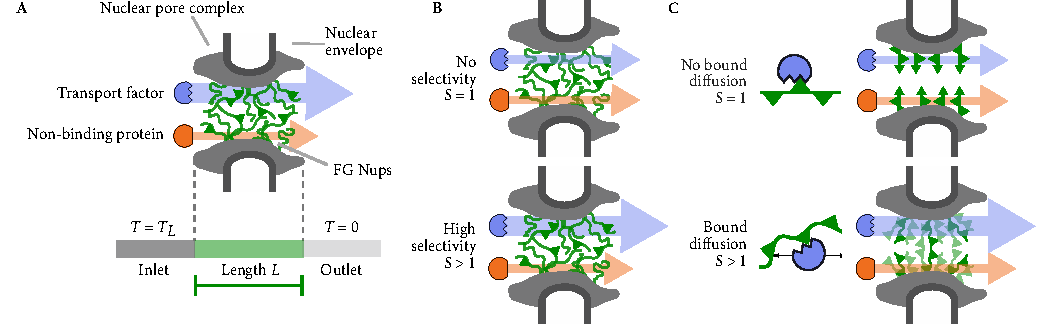
\includegraphics[width=17.8cm]{figs/ch02/fig1.pdf}
\caption{Schematics of the nuclear-pore complex and model. (A) The
  nuclear pore complex (gray) is filled with FG Nups (green polymers)
  that selectively passage transport factors that bind to FG Nups
  (blue) while blocking non-binding proteins (red). The central
  channel of the pore has length $L$. Protein concentration is high on
  the left (inlet) and low on the right (outlet).  (B) Selectivity
  quantifies the degree of selective transport through the pore. A
  non-selective pore with $S=1$ has the same flux for a transport
  factor as for a non-binding protein (top). A selective pore with
  $S>1$ has a larger flux for a transport factor than a non-binding
  protein (lower). (C) The bound diffusion coefficient quantifies the
  mobility of a bound transport factor.  A transport factor may be
  immobile (top) or mobile (lower) when bound. }
\label{fig:cartoon}
\end{figure*}

Models of the NPC selective barrier have proposed that the FG Nups may
form an entropic brush \cite{rout00}, a dynamic hydrogel
\cite{ribbeck01, frey07}, an intermediate state between a brush and
gel \cite{vovk16}, or liquid droplets \cite{schmidt15}.  These
mechanisms may be modulated by spatial organization \cite{yamada10,
  ando14} and binding of TFs to multiple FG repeats \cite{lowe15,
  schoch12}.  Attempts to distinguish these models have been hindered
by the pore's small size, the redundancy and multiple copies of FG
Nups, and contradictory experimental results on FG Nups and TF binding
\cite{vovk16}. Some FG Nup fragments form less-dynamic hydrogels
\vitro\ \cite{frey07}, but remain highly dynamic within cells
\cite{hough15}. Molecular dynamics simulations find highly dynamic FG
Nups, though the degree and extent of motion depends on the affinity
of FG repeats for each other and for TFs \cite{pulupa17,
  vovk16}. Crowding and competition modulate affinity
\cite{tetenbaum-novatt10} and may contribute to selective transport
\cite{zilman07}.  However, the connection between the amino-acid level
behavior of the FG-TF interaction and macroscopic transport
selectivity remains unclear.  Here we address the central
contradiction of selective transport through the NPC: how does binding
of TFs to FG Nups within the pore increase the flux rather than
decreasing it \cite{bickel02, witten17}?

Using a biophysical model, we demonstrate that TF diffusion and
binding are sufficient for selective transport, as long as binding
only partially immobilizes TFs. Binding increases the local
concentration, and these molecules contribute to the flux if mobile.
Thermally-driven diffusion of TFs bound to flexible tethers gives
sufficient particle mobility to produce selectivity similar to
experimental measurements.  Tether flexibility also allows bound TFs
to hop between tethers, further enhancing selectivity.

\section*{Biophysical model of transport through the NPC}

We consider a minimal model of the central channel of the NPC
containing FG Nups homogeneously anchored \figref{fig:cartoon}.  This
model is sufficiently general to describe the common features of a
range of biopolymer filters.  The NPC, unlike most other biopolymer
filters, has a wide capture area that may increase transport rates
\cite{pagliara14}.  In order to focus on basic principles of
transport, we neglect this effect.  A varying free energy landscape
along the axis of the NPC may play a role in selective transport
\cite{zilman07, tagliazucchi13, tu13, timney16}.  However, the NPC is
robust to deletion of all asymmetric Nups and many Nup combinations,
indicating that spatial variation in pore properties is not necessary
\cite{strawn04, zeitler04}.  Experiments \vitro\ with simplified,
homogeneous Nup composition produced selective transport
\cite{kowalczyk11, jovanovic-talisman09}.

\begin{figure*}[t!]
\centering
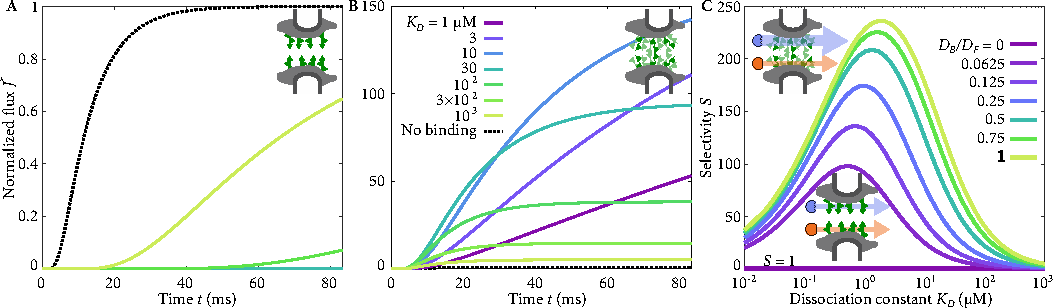
\includegraphics[width=\textwidth]{figs/ch02/fig2.pdf}
\caption{Flux through the pore and selectivity for TFs with varying
  bound mobility. (A) Flux as a function of time when TFs are immobile
  while bound, with varying binding affinity as in (B).  (B) Flux as a function
  of time when TFs are mobile while bound with $D_B = D_F$, with
  varying binding affinity.  (C) Selectivity as a function of
  dissociation constant with varying bound diffusion coefficient. }
\label{fig:transient}
\end{figure*}

Rapid transport requires TF-FG Nup binding, while a protein similar to
a TF but unable to bind FGs is excluded. Therefore, in our model we
compare two proteins that are identical, except that one binds FG Nups
and the other does not.  As a model TF, we consider nuclear transport
factor 2 (NTF2) \cite{ribbeck98}. NTF2 is small ($\sim$5 nm) relative
to the diameter ($\sim$50 nm) and length of the pore ($\sim$100 nm),
suggesting that passage of NTF2 does not require large-scale molecular
rearrangements that have been proposed for larger molecules
\cite{lowe15, frenkiel-krispin10}. Because of the small size of NTF2 we
neglect effects of steric crowding, which can enhance selectivity in a
transport model \cite{zilman07}.  NTF2 appears not to be actively
released from the pore, suggesting that selective transport is an
intrinsic property of the NPC \cite{mincer11, zilman07}, and in
contrast to actively released karyopherins \cite{lowe15, mincer11,
  gorlich96, gilchrist02}.

Transport through the NPC requires entry into the pore, passage, and
exit. In single-molecule measurements, most of the transport time is
spent in a random walk within the central channel \cite{yang04,
  tu13}. We therefore assume that entry and exit rates are determined
by binding kinetics (see Supporting Information, section
\ref{sec:entry} for the model when entry and exit are rate-limiting.)
The directional bias in TF transport is controlled outside the NPC
through a concentration difference between the nucleus and cytoplasm
generated by the Ran-GTP system \cite{riddick05}.  In our model, we
impose a fixed concentration difference across the pore.

We consider a channel of length $L$ filled homogeneously with Nups
that separates two reservoirs \figref[A]{fig:cartoon}.  Within the
channel are free transport factor (concentration $T$), free FG Nups
($N$), and bound TF-FG complex ($C$), with total Nup concentration
$N_t= N+C$.  TF diffusion within the channel ($0<x<L$) is described by
the reaction-diffusion equations
\begin{eqnarray}
  \frac{\partial T}{\partial t} &=& -\kon T N+\koff C +D_F
       \frac{\partial^2 T}{\partial x^2},\label{eq:continuum_main} 
   \\ 
  \frac{\partial C}{\partial t} &=& \kon T N -\koff C + 
        D_B \frac{\partial^2 C}{\partial x^2} .
\label{eq:continuum_main_2} 
\end{eqnarray}
TF-FG interaction has on-rate constant $\kon$, off-rate $\koff$, and
dissociation constant $K_D =\koff/\kon$.  We include competition
between TFs for FG binding sites \cite{timney16}.  The
diffusion constants of free ($D_F$) and bound ($D_F$) TFs are
spatially constant. The fixed reservoir TF concentrations are $T_L$
(inlet, left) and 0 (outlet, right).

The flux of transport factor out of the pore
$J = - D_F \left. \partial T/\partial x \right|_{x=L}$. We numerically integrated
the full equations.  Because flux
measured in experiments is typically linearly proportional to TF
concentration \cite{timney06, schmidt15}, TF concentration likely
remains below binding saturation in the NPC. Therefore, we also solved
eqns.~(\ref{eq:continuum_main}, \ref{eq:continuum_main_2})
analytically in the low binding limit.  We define
the transport selectivity $S$ as the ratio of steady-state flux of a
binding versus a non-binding species \figref[B]{fig:cartoon}
\begin{equation}
  S =  \frac{J_{\rm binding}(t \to \infty)}{J_{\rm non-binding}(t \to \infty)} .
\end{equation}

\subsection*{No selective transport occurs if bound TFs are immobile}
If TF-FG Nup binding immobilizes the TF, the bound-state diffusion
coefficient $D_B = 0$.  For immobile bound TFs, transport is not
selective: the steady-state flux $J = D_F T_L/L $ for both binding and
non-binding proteins, so $S = 1$ (figs.~\ref{fig:transient},
\ref{fig:linear-selectivity}).  The binding TF accumulates within the
pore, but its immobility means it does not enhance transport compared
to the non-binding case.  Notably, this effect is independent of
binding kinetics.  Prior to steady state, binding slows transport
\figref[A]{fig:transient}.  In systems such as airway mucus,
immobilization may increase the time available for degradation or
active clearance, consistent with the observation that binding tends
to inhibit selective transport in those systems \cite{schneider17,
  huang17, mastorakos15}.  This effect is related to the binding-site
barrier seen in antibody delivery to tumors \cite{juweid92}, and
observations that non-binding nanoparticles are often more effective
in drug delivery to tumors than binding particles \cite{witten17}.

Our model is related to the classic problem of molecular transport
through an oil membrane separating two aqueous reservoirs
\cite{schafer13}.  The relative concentration of a species just inside
the oil barrier to the concentration in water is called the partition
coefficient.  The steady-state flux through the membrane is directly
proportional to the partition coefficient (Supporting Information,
section \ref{sec:partition}, fig.~\ref{fig:oil-membrane}).  By
analogy, one might expect the TF-FG binding affinity to determine the
flux across the pore. However, binding is different from partitioning.
In systems where the increase in intra-pore concentration arises from
binding, the effective diffusion coefficient is typically inversely
proportional to the partition coefficient, making the flux independent
of binding affinity \cite{bickel02}.  This result led us to consider
whether TFs may be mobile while bound to FG Nups.

\begin{figure*}
\centering
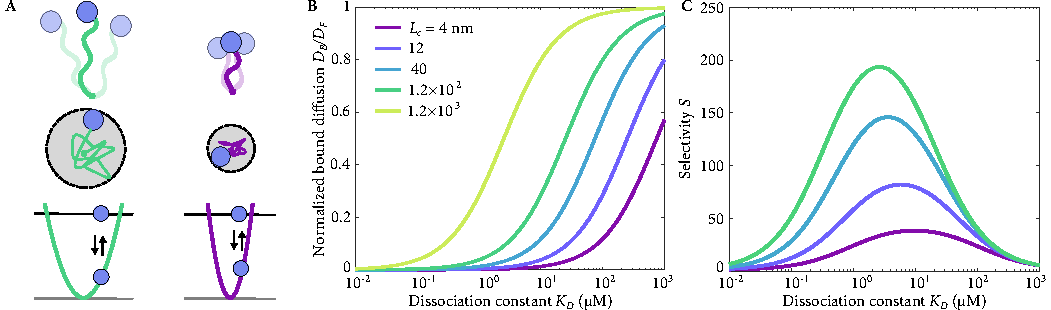
\includegraphics[width=\textwidth]{figs/ch02/fig3.pdf}
\caption{(A) Schematic of the flexible tether model of bound-state
  diffusion. FG Nups are treated as entropic springs that constrain
  the motion of TFs more (top and center left, longer FG Nup) or less
  (top and center right, shorter Nup), which corresponds to changing
  width of the harmonic potential well (lower).  (B) Ratio of bound to
  free diffusion coefficient as a function of dissociation constant,
  with varying polymer length in the tethered-diffusion model.  (C)
  Selectivity as a function of $K_D$, with varying polymer length in
  the tethered-diffusion model.}
\label{fig:tethers}
\end{figure*}


\subsection*{Bound-state diffusion allows selective transport}
When bound TFs are mobile, selective transport occurs with a
selectivity up to 240 for a conservative set of parameters
(figs.~\ref{fig:transient}B,C, \ref{fig:linear-selectivity},
Supporting Information, section \ref{sec:param}).  Remarkably, this
selectivity is comparable to experimental measurements of NTF2 versus
GFP flux (Table \ref{table:NTF2-flux}).  The interplay between binding
kinetics and diffusion leads to an optimal dissociation constant
$\sim$1 $\mu$M for maximum selectivity \figref[C]{fig:transient}.
Selectivity decreases for high $K_D$ because binding is too weak to
significantly increase TF concentration in the pore.  For low $K_D$,
tight binding causes the concentration of bound complexes to become
approximately constant across the pore. Because diffusive flux is
driven by a concentration gradient, this washing out of the gradient
by tight binding decreases flux and selectivity.

\begin{table}[b!]
  \caption{Comparison between experimental results for NTF2 and GFP
    (a similarly-sized non-binding protein) and model
    predictions. Flux measured in units of molecules per pore per
    second.}
    \label{table:NTF2-flux}
    \begin{tabular}{p{2.1cm}p{1.2cm}p{1.7cm}p{0.9cm}p{1.6cm}p{0.8cm}}
      Method & Cell type & Species & Flux & Selectivity & Notes\\
      \hline
      OSTR & \textit{Xenopus} & \makecell[cl]{NTF2\\GFP} & \makecell[cl]{91--123\\3.3--3.8} & 24--37 
                         &\cite{siebrasse02}
      \\
      OSTR & \textit{Xenopus} & \makecell[cl]{NTF2\\GFP} & \makecell[cl]{47.3\\1.1} & 43 &  \cite{kiskin03}\\
      \makecell[cl]{Permeabilized \\ cells}  & HeLa &
                                                    \makecell[cl]{NTF2\\GFP} & \makecell[cl]{250\\2} & 125 & \cite{ribbeck01}\\
      Model & -- & \makecell[cl]{Binding\\Non-binding} & \makecell[cl]{2--480\\2} & 1--240 & \makecell[cl]{This\\work}\\
    \end{tabular}
\end{table}

Our model predicts that selectivity is increased by increasing binding
on-rate constant $\kon$ \figref{fig:parameter-variations}. Consistent
with this, the on-rate constants of TF-FG Nup interactions have been
measured to be diffusion limited \cite{milles15, hough15}.  Large
$\kon$ makes transport more selective because fast binding kinetics
relative to diffusive motion are necessary to maintain steep
concentration gradients within the pore. High FG Nup concentration (as
measured experimentally) leads to large $N_t$ and low $D_F$, both of
which increase selectivity.  Decreasing $D_F$ or increasing the length
of the pore both reduce the magnitude of the flux and increase
selectivity (figs.~\ref{fig:parameter-variations},
\ref{fig:parameter-variations-abs-flux}). Therefore, varying TF free
diffusion coefficient and pore length involves a trade-off between
transit time and selectivity.


\section*{Mechanisms of  bound transport factor mobility}

Our result that bound-state diffusion is required for selective
transport raises a mechanistic question: how can TFs move while bound
to FG Nups? Here we consider two experimentally based mechanisms:
movement of the bound TF due to the intrinsic flexibility of the FG
Nups \cite{patel07} and multivalent binding that allows hopping of TFs
between neighboring Nups \cite{raveh16}.

\subsection*{FG Nup flexibility allows tethered diffusion}
Previous measurements have found that FG Nups are flexible and dynamic
\cite{lim07, milles14, hough15}. Although FG Nups are attached at one
end to the inner surface of the NPC scaffold, chain flexibility allows
a  TF bound far from the tethered end to move.  Flexible polymers
behave as entropic springs \cite{howard01} if they are not highly
stretched. Therefore, a bound TF diffuses while attached to a
spring-like tether, which can be represented as diffusion in a
harmonic potential well \figref[A]{fig:tethers}.  The width of the
harmonic well is related to the effective length of the flexible
domain: if FG Nups are not crosslinked, the effective length is the full FG Nup
length, while if they are crosslinked or entangled, the length is
reduced \cite{ribbeck01}.  The probability density of a TF that binds
to the center of a well at $x=0$ is
$P(x,t) = e^{-\frac{x^2}{2 \alpha(t)}}/\sqrt{2\pi \alpha(t)}$, where
$ \alpha(t) = (1-e^{-2kD_F\beta t})/(k\beta)$, $k$ is the spring
constant of FG Nup tethering and $1/\beta = k_BT$ is the thermal
energy \cite{cau12}.  The TF mean-squared displacement (MSD) is then
$\ev{x^2(t)} = \int_{-\infty}^{\infty} P(x,t) x^2 dx = \alpha(t)$.
The typical TF MSD during a binding event can be determined from the
probability density of binding time
$\rho (t) = \exp(-t/\tau)/\tau$, where $\tau = 1/\koff$ is the mean
bound lifetime:
\begin{equation}\label{eq:sho}
  \overline{\ev{x^2}} = \int_0^{\infty} \rho(t') \ev{x^2(t')} dt' = \frac{2D_F L_c
    \ell_p}{L_c \ell_p \koff+ 3D_F}. 
\end{equation} 
Here we assume that the spring constant is that of a worm-like chain
polymer $k = 3/(2\beta L_c \ell_p)$, where $L_c$ is the contour length
and $\ell_p$ the persistence length \cite{howard01}.

Because FG-TF interactions have fast binding kinetics \cite{milles15,
  hough15}, we estimate the bound diffusion coefficient by averaging
over many binding events, while considering only bound motion, giving
\begin{equation}\label{eq:dbound}
  D_B \approx \frac{\overline{\ev{x^2}}}{2\tau} = \frac{D_F L_c \ell_p
    k_\un{off}}{L_c \ell_p k_\un{off} + 3D_F} =
  \frac{D_F}{1+3\frac{D_F}{D_{P}}}.  
\end{equation}
Here $D_P = L_c \ell_p k_\un{off}$ controls the bound-state diffusion
coefficient: higher $D_P$ corresponds to a lower constraint of the TF
by the tether and greater bound mobility. Bound mobility increases
with increasing chain length, flexibility of the polymer, or
decreasing binding lifetime. When $D_P$ is large ($D_F/D_P\ll1$),
$D_B$ approaches $D_F$, since the long, flexible chains barely affect
TF motion during the short binding event. For small $D_P$
($D_F/D_P\gg1$), TF motion is inhibited by a short tether, giving
$D_B\approx D_P/3\ll D_F$.  This result highlights that the kinetics
of TF-FG Nup interaction are a primary determinant of the bound
mobility: the faster the binding kinetics, the higher the bound
diffusion constant.

\begin{figure*}
\centering
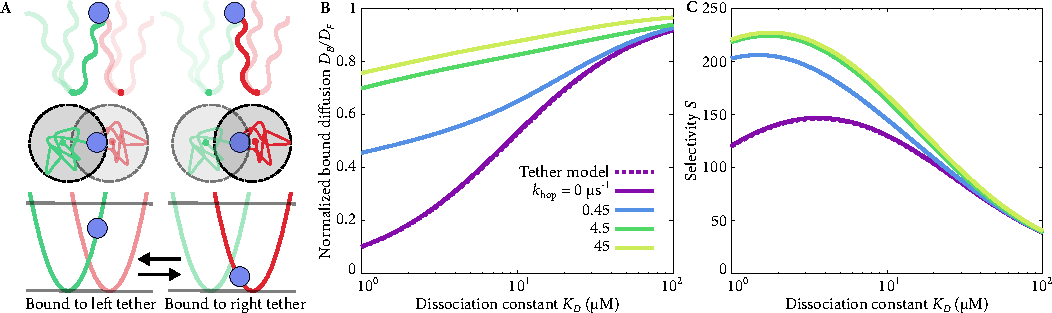
\includegraphics[width = \textwidth]{figs/ch02/fig4.pdf}
\caption{(A) Schematic of the inter-chain hopping model of bound-state
  diffusion. FG Nups are treated as entropic springs that constrain
  the motion of TFs, and inter-chain hopping allows a TF to move from
  one FG Nup (top and center left, green Nup) to another (top and
  center right, red Nup) without unbinding, which corresponds to
  switching from one harmonic potential well to another (lower). (B)
  Ratio of bound to free diffusion coefficient as a function of
  dissociation constant, with varying hopping rate in the inter-chain
  hopping model.  (C) Selectivity as a function of $K_D$ with varying
  hopping rate. FG Nup contour length $L_c = 40$ nm in (B, C). }
\label{fig:hopping}
\end{figure*}


Flexible disordered proteins typically have low persistence lengths
\cite{receveur-brechot12}, so we estimate $\ell_p \approx 1$ nm.  If
the on-rate constant is diffusion limited,
$\kon = 10^{-3}\mu \tx{M}^{-1} \, \mu \tx{s}^{-1}$ \cite{milles15,
  hough15}, the binding affinity determines the off rate.  Disordered
FG Nups have $L_c\approx$ 100--280 nm (250--700 amino acids long
\cite{patel07} with a contour length per amino acid $\approx 0.4$
nm). For our conservative parameters, tethered diffusion alone
predicts significant selectivity $\sim$200.

\subsection*{Inter-chain hopping increases selectivity}
The tethered diffusion mechanism is constrained by a trade-off:
tighter binding increases the TF concentration in the pore, but
hinders motion.  Multivalent TF-FG interactions can relax this
constraint, because a TF can bind simultaneously to more than one FG
Nup, moving hand-over-hand while remaining bound
\cite{tetenbaum-novatt12}. Consistent with this, TFs may slide between
nearby FG sites rather than fully unbinding and re-binding
\cite{raveh16}. If the newly-bound FG repeat is on a neighboring
chain, the FG tether site that constrains TF motion moves while the TF
remains bound.  We model inter-chain hopping with a TF that undergoes
tethered diffusion when bound to an FG Nup and hops between
neighboring, randomly distributed tethers \figref{fig:hopping}.
Numerical simulations of this model determined the bound diffusion
coefficient (fig.~\ref{fig:integrand}, Supporting Information, section
\ref{sec:sim}). We note that intra-chain hopping does not change the
flux, since the anchor point of the tethering chain is not changed;
therefore we neglect it.

Inter-chain hopping increases selectivity most for tight binding and
short chains, the parameter regime where tethered diffusion gives
limited selectivity (figs.~\ref{fig:hopping}, \ref{fig:partitioningB},
\ref{fig:partitioningC}). Hopping may therefore be important for FGs
that form transient crosslinks: if FG Nups are highly crosslinked, our
model suggests that inter-chain hopping is the key mechanism of TF
movement.  For weaker binding and longer chains, inter-chain hopping
leads to a modest increase in selectivity.

\section*{Discussion}

A key puzzle of the NPC is how transport-factor binding allows rapid
transport through the pore.  Binding typically immobilizes the bound
particle, and so the increase in concentration resulting from binding
does not, in general, result in increased flux. The biophysical theory
we developed includes diffusion of TFs due to thermal fluctuations,
binding to polymeric tethers, and the hopping of bound species between
these tethers.  Thus we identified principles of selective transport
resulting from binding \figref{fig:cartoon}, emphasizing that
bound-state mobility is essential for selective transport
\figref{fig:transient}.  Binding increases the local concentration,
and any bound mobility increases the flux.  We characterized two
mechanisms to obtain bound-state mobility and found that
thermally-driven diffusion of TFs bound to flexible tethers and rapid
binding kinetics \cite{hough15, milles15} allow TF mobility, leading
to selectivity similar to that observed experimentally
\figref{fig:tethers}.  In addition, tether flexibility enables
multivalent bound particles to hop between binding regions
\figref{fig:hopping} \cite{lowe15, schoch12}, further enhancing
selectivity. Mobility of bound or partitioned molecules occurs in many
biological contexts, suggesting that the mechanisms we study here may
be broadly applicable \cite{stefferson17, braga07}.


Our model for selective transport by tethered diffusion generalizes to
a range of FG-FG interactions \cite{vovk16}, if we decrease the
effective chain length $L_c$ for cohesive FG Nups.  For short chains
the selectivity simply due to chain flexibility is modest, suggesting
that other mechanisms, like hopping, may be important.  Our model
suggests that transient cross-linking of FG repeats proposed to occur
within the pore may serve to increase the viscosity and therefore the
selectivity. Crosslinks need not be actively melted by TFs to enhance
selectivity \figref{fig:parameter-variations}.
  
Our model provides a quantitative tool to evaluate selective
transport. Materials formed \textit{in vitro} by spontaneous
self-assembly of FG Nups \cite{frey07} or transient crosslinking by
alpha-helical peptides \cite{kim15} show strong selective
\textit{entry}.  Using published data, we predicted whether these gels
also showed selective \textit{transport} (table \ref{table:Gorlich}).
Most synthetic gels are predicted to have $S<10$, less than the
selectivity of NTF2 in cells (table \ref{table:NTF2-flux}). The
predicted selectivity of one hydrogel is $S\approx200$, apparently the
most selective synthetic gel to date \cite{frey07}.


\subsection*{Overcoming the limitations of binding}
Binding, even in the presence of bound-state motion, limits
selectivity.  Biological systems appear to have developed strategies
to avoid this, for example, by using true partitioning.  Lipid domains
in complex membranes partition proteins \cite{simons11}.  Membraneless
organelles spontaneously assembled from low-complexity proteins and
nucleic acids can localize a molecule without immobilizing it
\cite{brangwynne15}.  Because membraneless organelles are fluid, the
constraints imposed in our NPC model by binding are released.  Our
work thereby suggests a benefit of phase-separated droplets to cells:
they provide significantly higher selectivity than can occur with
immobilizing binding. This may be especially important for spatially
complex assemblies \cite{feric16}.

Though we show it is not necessary, the active dissolution of
polymeric biomaterials has been proposed to occur in the NPC
\cite{ribbeck01}. This strategy is used by \textit{Helicobacter
  pylori} to penetrate the gastric mucus \cite{celli09}. Because the
particularly dense extracellular matrix of solid tumors blocks the
motion of particles, especially larger nanoparticles, ECM dissolution
has been used to enhance drug delivery \cite{zhou13}. Unfortunately,
this approach may not be universally applicable: breaking down the ECM
surrounding tumors may promote cancer metastasis \cite{miao15}.

\subsection*{Design principles of selective transport by binding}

Filtering by polymeric biomaterials occurs in many systems for
particles of different sizes: for example, nutrients reach our
intestinal walls while larger molecules are excluded.  However,
controlling the selective transport of similarly-sized molecules by
tuning specific interactions has proven elusive. In drug delivery
applications, inert nanoparticles are typically more effective at penetrating
extracellular spaces and reaching their cellular targets
\cite{witten17}. Because biopolymer filters are the first point of
contact of nanoparticles used for drug delivery, specific targeting of
transport through mucus may enhance the effectiveness of drug
delivery. If NPC-like bound mobility as described in our model could
be achieved in these systems, it would increase the rates of
transport and drug delivery. 
